\documentclass[10pt,twocolumn,letterpaper]{article}

\usepackage{acvs}
\usepackage{times}
\usepackage{epsfig}
\usepackage{graphicx}
\usepackage{amsmath}
\usepackage{amssymb}

% Include other packages here, before hyperref.
\usepackage{dsfont}

% If you comment hyperref and then uncomment it, you should delete
% egpaper.aux before re-running latex.  (Or just hit 'q' on the first latex
% run, let it finish, and you should be clear).
\usepackage[pagebackref=true,breaklinks=true,letterpaper=true,colorlinks,bookmarks=false]{hyperref}

\iccvfinalcopy % *** Uncomment this line for the final submission

\def\iccvPaperID{} % *** Enter the Paper ID here
\def\httilde{\mbox{\tt\raisebox{-.5ex}{\symbol{126}}}}

% Pages are numbered in submission mode, and unnumbered in camera-ready
\ificcvfinal\pagestyle{empty}\fi

\begin{document}

%%%%%%%%% TITLE - PLEASE UPDATE
\title{End-to-End Object Detection with Transformers~\cite{detr} \\ {\rm {\normalsize Minji Kim (minji@snu.ac.kr; 2020-28702), Dept. of Electrical and Computer Engineering, Seoul National University}}}   % **** Enter the paper title and student information here

\maketitle
\thispagestyle{empty}

%%%%%%%%% BODY TEXT - ENTER YOUR RESPONSE BELOW

%%%%%%%%%%%%%%%%%
%%%%%%%%%%%%%%%%%
\section{Introduction}
Previous modern object detectors such as Faster R-CNN~\cite{fasterrcnn} require hand-crafted components such as pre-defined anchor generation and non-maximum suppression (NMS) post-processing.
Such pipelines are not fully end-to-end and require manual hyper-parameter adjustment for each dataset.
To address this issue, this paper suggests a new detection method, called DEtection Transformer (DETR), which sees object detection as a direct set prediction problem.
DETR predicts all objects at once based on end-to-end training with a set loss function which helps bipartite matching between prediction and ground-truth objects.



%%%%%%%%%%%%%%%%%
%%%%%%%%%%%%%%%%%
\section{DETR}
% \subsection{Subsection}
% Paper reference should be like \cite{wug2018fast}.

%%%%%%%%%%%%%%%%%
\subsection{Architecture}
DETR consists of three main component: a CNN backbone to extract a feature representation, an encoder-decoder transformer, and a lightweight feed forward network (FFN) that generates the final detection prediction.
The overall pipeline is illustrated in Fig.~\ref{fig:overview}.
DETR first extracts a 2D feature representation from a standard CNN backbone.
The flattened feature is combined with a positional encoding and passes through a transformer encoder.
Along with the encoded features, a transformer decoder takes as input a small fixed number of learned positional embeddings, called \textit{object queries}, resulting the decoded features where the positional and semantic information are attended.
Finally, each output embeddings of the decoder passes through a shared feed forward network (FFN) that predicts class, bounding box, with a ``no object'' class.


%%%%%%%%%%%%%%%%%
\subsection{Object Detection Set Prediction Loss}
Given $y$ the ground truth set of objects and the set of $N$ predictions $\hat{y}=\{\hat{y}_i\}^N_{i=1}$, we find a bipartite matching by searching for a permutation of $N$ elements $\sigma \in C_N$ with the lowest cost:
%
\begin{equation}\label{eq:matching}
    \hat{\sigma}={\arg\min}_{\sigma \in C_N}\sum^N_i{\mathcal{L}_{match}(y_i, \hat{y}_{\sigma(i)})},
\end{equation}
%
where $\mathcal{L}_{match}(y_i, \hat{y}_{\sigma(i)})$ is a pair-wise matching cost between ground truth $y_i$ and a prediction with index $\sigma(i)$.
Here, each element $i$ of the ground truth set is $y_i=(c_i, b_i)$ where $c_i$ is the target class label (including no-object) and $b_i\in[0,1]^4$ that represents a relative coordinate and size of a bounding box.
This matching procedure plays same role with the previously used proposal matching or anchors, but the main difference is that in this scenario the matching should be one-to-one without any duplication.
Finally, the Hungarian loss for all matched pairs can be obtained as follows:

\begin{equation}\label{eq:loss}
    \mathcal{L}(y,\hat{y})
    =\sum^N_{i=1}{[-\log \hat{p}_{\hat{\sigma}(i)}(c_i)
    + \mathds{1}_{c_i\neq \emptyset}\mathcal{L}_{box}(b_i, \hat{b}_{\hat{\sigma}}(i))]},
\end{equation}

where $\hat{\sigma}$ is the optimal assignment found in the previous step.
The bounding box loss $\mathcal{L}_{box}$ is a linear combination of the $l_1$ loss and the generalized IoU loss~\cite{giou}.





%%%%%%%%%%%%%%%%%
%%%%%%%%%%%%%%%%%
\section{Discussion}
DETR is the first detection framework to integrate Transformers into the detection pipeline. It eliminates the burdensome hand-craft components of previous detection frameworks.
In experiments on COCO~\cite{coco} dataset, it achieves competitive performance with previous modern object detectors such as Faster R-CNN.
However, the convergence of DETR is 10x~20x slower than Faster R-CNN, and its feature resolution is limited, showing limited performance compared to the Faster R-CNN with FPN setting.




\begin{figure}[t]
    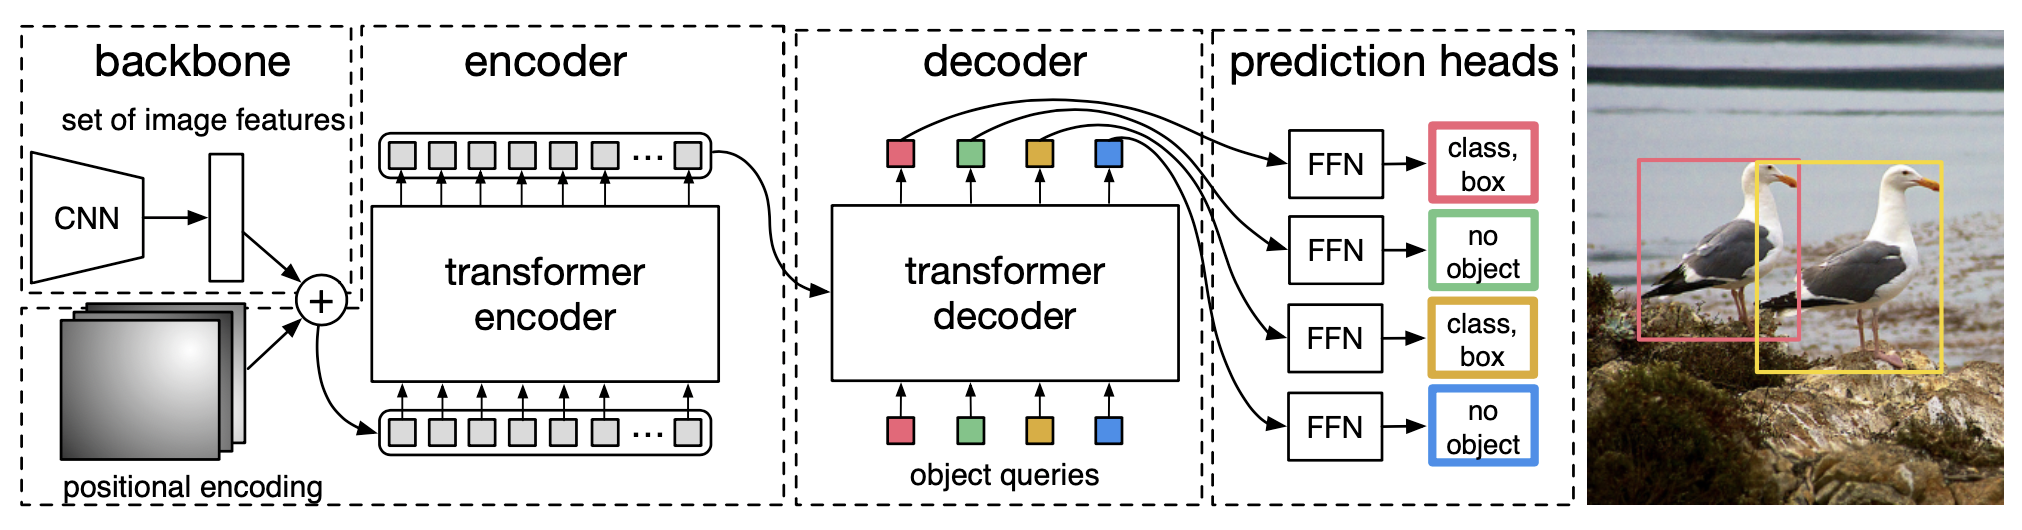
\includegraphics[width=\linewidth]{assets/detr.png}
    \caption{\label{fig:overview}The overall pipeline of DETR. DETR consists of CNN backbone, encoder-decoder for transformer, and multiple prediction heads with shared feed-forward networks.}
\end{figure}


{\small
\bibliographystyle{ieee}
\bibliography{egbib}
}

\end{document}
